\chapter{API}
\label{sec:module.API}

Unsere AITools API dient als Grundbaustein des gesamten Projekt. Sie entkapselt die Interfaces zu unseren Search- und Strategieimpelementierungen. Sie beinhaltet zudem Basisklassen, welche �berall verwendet werden. Der Inhalt ist wie folgt:

\section{Entities}
\label{sec:mocule.API.Entities}

\begin{figure}[H]
\centering
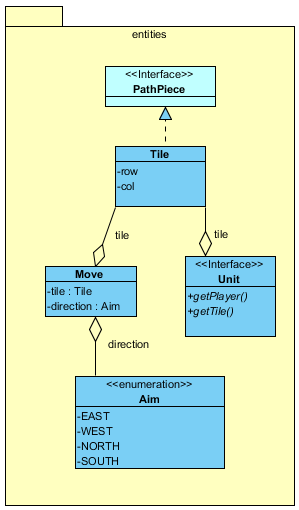
\includegraphics[width=0.5\textwidth]{91_bilder/apiEntities}
\caption{Entities}
\label{fig:apiEntities}
\end{figure}

\begin{itemize}
\item
\textbf{Aim}: Richtungangabe zum Beschreiben einer Bewegung der Ameise
\item
\textbf{Tile}: Repr�sentiert eine Zelle auf dem Spielfeld, welche mit Row (Zeile) und Column (Spalte) beschrieben ist.
\item
\textbf{Move}: Diese Klasse beschreibt einen Spielzug mit den Eigenschaften Tile, von wo aus der Zug statt findet, und Aim, in welche Richtung der Zug ausgef�hrt wird.
\item
\textbf{Unit}: Unit besteht aus Tile und Spieler und definiert eine Einheit eines Spielers auf der Karte.
\end{itemize}

\section{Map}
\label{sec:mocule.API.Map}

\begin{figure}[H]
\centering
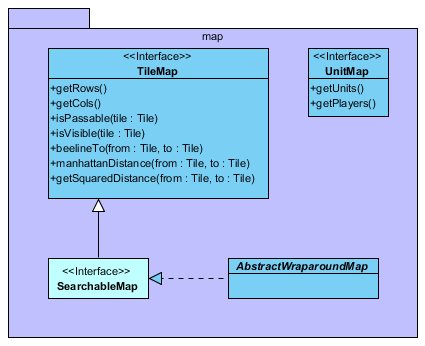
\includegraphics[width=0.7\textwidth]{91_bilder/apiMap}
\caption{Map API}
\label{fig:apiMap}
\end{figure}

\begin{itemize}
\item
\textbf{TileMap}:  Dieses Interface definiert, welche Methoden eine auf Tiles aufbauende Spielkarte anbieten muss. Dazu geh�ren die Masse der Karte, ob ein Tile auf der Karte sichtbar und passierbar ist, sowie Distanz Messfunktion wie ManhattanDistanz, Luftlinie, quadrierte Distanz.
\item
\textbf{UnitMap}: UnitMap ist auch ein Interface welches auf TileMap aufbaut und zus�tzlich die Methoden definiert die Einheiten und Spieler zur�ckzugeben.
\item
\textbf{AbstractWraparoundMap}: Implementiert das Interface SearchableUnitMap (siehe: Abschnitt Search). Hier sind alle Methoden implementiert, welche die Karte anbieten muss, damit sie mit den Suchalgorihmen verwendet werden kann. Zudem sind die Methoden aus TileMap implementiert. Diese geben �ber die Gel�ndebeschaffenheit und Distanzen Auskunft.
\item
\textbf{WorldType}: WorldType ist ein Enum und definiert die Art der Karte. Der Typ Globus hat keine Kartenr�nder, ist also ringsum begehbar. Von diesem Typ ist auch die Ants Challenge somit auch die Klasse AbstractWraparoundMap. Der zweite Enumtyp ist Pizza und definiert eine Welt so wie unsere Erde vor 500 Jahren noch definiert wurde, eine Scheibe mit R�ndern, welche die Welt begrenzen. Dieser zweite Typ wurde provisorisch erstellt. Falls diese API eine Weiterverwendung findet, kann dieser Typ zus�tzlich implementiert werden.
\end{itemize}


\section{Search}
\label{sec:mocule.API.Search}

\begin{figure}[H]
\centering
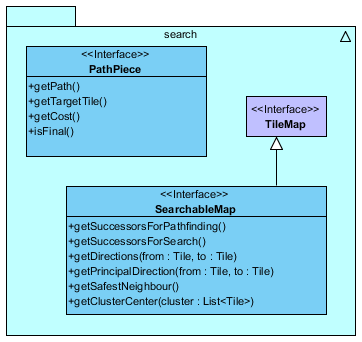
\includegraphics[width=0.6\textwidth]{91_bilder/apiSearch}
\caption{Search API}
\label{fig:apiSearch}
\end{figure}

\begin{itemize}
\item
\textbf{PathPiece}: Das PathPiece ist ein Interface f�r Strukturen, die als Suchknoten in der Pfadsuche verwendet werden k�nnen. Es definiert die f�r die Suche n�tigen Methoden, wie getSuccessors(), getCost(), oder getPath(). 
Implementierende Klassen sind Edge (rep�sentiert eine Kante in einem Cluster) und Tile. Erweiterungen dieser Klassen sind DirectedEdge (eine gerichtete Kante) und Vertex (eine Zelle mit zugeh�rigen Kanten).
\item
\textbf{SearchableMap}: Das Interface SearchableMap erweitert das Interface TileMap. Es beschreibt die Methoden zur Pfadsuche.
\item
\textbf{SearchableUnitMap}: Dieses Interface dient ausschliesslich zur Zusammenf�hrung der beiden Interfaces UnitMap und SearchableMap.
\end{itemize}

\section{Strategy}
\label{sec:mocule.API.Strategy}

\begin{figure}[H]
\centering
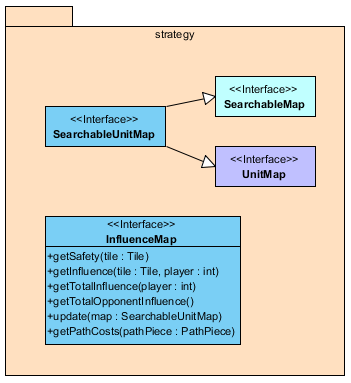
\includegraphics[width=0.6\textwidth]{91_bilder/apiStrategy}
\caption{Strategy API}
\label{fig:apiStrategy}
\end{figure}